\begin{figure}[t]
  \centering
  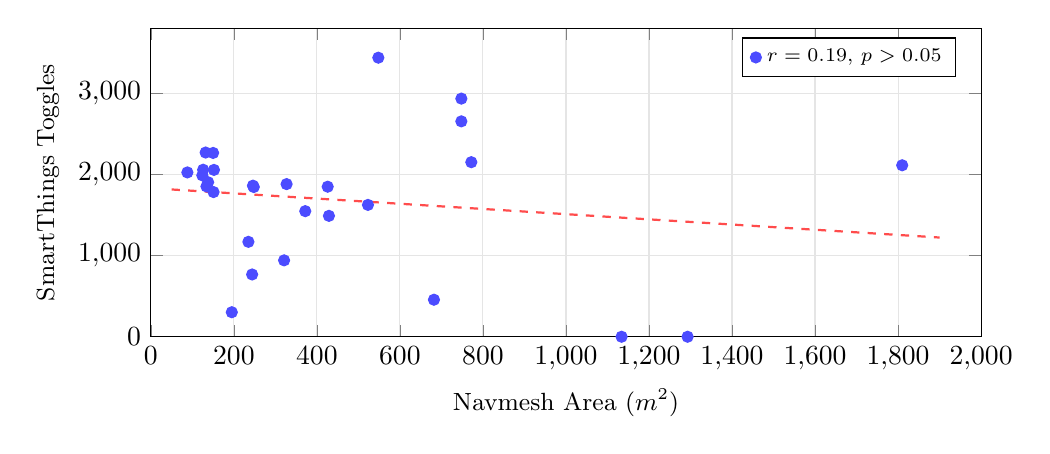
\begin{tikzpicture}
    \begin{axis}[
      width=\columnwidth,
      height=5.5cm,
      xlabel={Navmesh Area ($\text{m}^2$)},
      ylabel={SmartThings Toggles},
      ylabel style={font=\small},
      xlabel style={font=\small},
      xmin=0, xmax=2000,
      ymin=0, ymax=3800,
      grid=major,
      grid style={gray!20},
      legend style={at={(0.97,0.97)}, anchor=north east, font=\scriptsize},
    ]
    % Scatter points from per-scene data (28 scenes)
    \addplot[only marks, mark=*, blue!70, mark size=2pt] coordinates {
      (1810, 2112) (138, 1903)  (682, 456)   (1293, 0)
      (150, 2264)  (132, 2269)  (426, 1848)  (429, 1489)
      (244, 767)   (321, 941)   (548, 3437)  (248, 1844)
      (772, 2150)  (327, 1880)  (88, 2024)   (523, 1624)
      (124, 1988)  (372, 1547)  (748, 2933)  (1134, 0)
      (126, 2057)  (246, 1861)  (151, 1782)  (195, 302)
      (235, 1169)  (134, 1852)  (748, 2653)  (152, 2055)
    };

    % Regression line
    \addplot[red!70, thick, dashed, domain=50:1900, samples=2]
      {-0.32*x + 1830};
    \addlegendentry{$r = 0.19$, $p > 0.05$}

    \end{axis}
  \end{tikzpicture}
  \caption{Navmesh area vs.\ SmartThings proximity toggles across
  28~scenes.  Per-scene toggle count correlates strongly with
  device count ($r = 0.96$, $p < 0.001$) rather than navmesh area
  ($r = 0.19$, $p > 0.05$), indicating that device density---not
  floor plan compactness---drives interaction frequency.}
  \label{fig:scatter-toggles}
\end{figure}
